%% Computational Materials Science -- Elsevier elsarticle format
\documentclass[preprint,12pt,authoryear]{elsarticle}

\usepackage{cmap}
\usepackage[T1]{fontenc}
\usepackage{lmodern}
\usepackage[utf8]{inputenc}
\usepackage{amsmath,amssymb}
\usepackage{graphicx}
\usepackage{booktabs}
\usepackage{array}
\usepackage{multirow}
\usepackage{xcolor}
\usepackage[hidelinks]{hyperref}
\usepackage{lineno}

\journal{Computational Materials Science}

\newcommand{\Np}[1]{N^{#1}}
\newcommand{\Dk}{\Delta^{K-1}}

\begin{document}

\begin{frontmatter}

\title{Simplex Constraints, Spatial Generalization, and the
Regressor--Detector Gap in Machine-Learning Surrogates for CALPHAD
Phase-Fraction Prediction}

\author[a]{Anonymous}
\address[a]{Anonymous}

\begin{abstract}
Surrogate models that map composition and temperature to equilibrium phase
fractions must respect the simplex constraint $\sum_k \Np{k} = 1$, yet the
literature offers no consensus on how that constraint should be imposed. We
compare six output heads --- sigmoid, softmax, sigmoid/$\Sigma$,
clip-then-renormalise, sparsemax, and a residue closure head --- against
four classical baselines across five Fe-based ternary systems (Fe--Cr--Ni,
Fe--Cr--Mn, Fe--Cr--Mo, Fe--Cr--V, Fe--Mn--Ni) solved with pycalphad from
the open MatCalc steel database, totalling 44{,}397 mass-balance-validated
equilibria; power normalisation and a sum-to-one loss penalty are
evaluated additionally as mechanism probes on Fe--Cr--Ni. Structurally
constrained heads satisfy sum-to-one closure to $\le 5\times10^{-8}$ at no
accuracy cost; the unconstrained sigmoid violates it by 6--8\%, and the
residue head, which enforces closure but not non-negativity, produces
negative fractions on up to 1.2\% of cells. No single evaluated
architecture consistently dominates across the five systems: constrained
multilayer perceptrons lead on systems with dense smooth coexistence
(Fe--Cr--Ni, Fe--Cr--Mn), while random forests win where sharp phase
boundaries dominate (Fe--Cr--V, Fe--Mn--Ni), and paired-bootstrap tests
confirm the two near-ties. Two spatial protocols, each with a size-matched
random control, separate \emph{where} points are held out from the penalty
of having less data. On contiguous interior holdout bands --- which a
Delaunay check shows to lie 99.3--99.4\% inside the convex hull of the
remaining training points --- the random forest pays a $3.11\times$ penalty
against $1.61\times$ for the constrained MLP on the Fe--Cr--Ni composition
band, whereas on the temperature band both pay $1.31\times$: constrained
MLPs degrade more gracefully than trees under contiguous composition-region
holdout. Under strict one-sided out-of-range extrapolation along a single
coordinate (train $x_2 \le 0.25$, test $x_2 > 0.35$; train $T \le 1200$~K,
test $T > 1400$~K) all evaluated model families degrade sharply, and the
constrained MLP achieves the lowest absolute far-side error in all five
systems, although absolute extrapolation performance remains poor.
Phase-presence detection degrades faster than regression under distribution
shift: $F_1$ collapses on the held-out temperature band for all evaluated
models even where MAE barely moves, and the qualitative regressor--detector
gap is stable across presence thresholds $10^{-4}$--$10^{-2}$, although the
detector ranking flips with the threshold on Fe--Cr--Mo. Three negative
results are
reported in full: under the evaluated configuration sparsemax exhibits
severe seed sensitivity; a sum-to-one penalty degrades MAE by
8--16$\times$; and the residue head is 1.3--2.5$\times$ worse than the best
constrained head in all five systems.
\end{abstract}

\begin{keyword}
CALPHAD \sep surrogate model \sep phase fraction \sep simplex constraint \sep
spatial generalisation \sep iron alloys
\end{keyword}

\end{frontmatter}

\linenumbers

% ======================================================================
\section{Introduction}
\label{sec:intro}

\subsection{Phase fractions as a regression target}

The CALPHAD method predicts equilibrium phase assemblages from assessed
thermodynamic databases \citep{saunders1998calphad,lukas2007computational}.
Given a database, the equilibrium at fixed composition $\mathbf{x}$,
temperature $T$ and pressure $P$ follows from constrained Gibbs-energy
minimisation, and the output of interest in alloy design is frequently the
vector of phase fractions $\mathbf{y} = (\Np{1}, \ldots, \Np{K})$, where
$K$ is the number of phases that can appear. This vector lies on the
probability simplex,
\begin{equation}
    \mathbf{y} \in \Dk, \qquad
    \sum_{k=1}^{K} \Np{k} = 1, \qquad \Np{k} \ge 0,
    \label{eq:simplex}
\end{equation}
by the mass balance of the equilibrium solver. Any surrogate that predicts
$\mathbf{y}$ should respect Eq.~\eqref{eq:simplex}; a prediction that
violates it is not merely inaccurate but physically inadmissible.

Machine-learning surrogates replace the per-point minimisation with a forward
pass \citep{hart2021fast}. Surrogates of phase-equilibrium and
quasi-equilibrium calculations have been developed for process optimisation
and phase-field coupling \citep{nentwich2019surrogate,jiang2019fast},
deep-learning surrogates now reproduce CALPHAD phase fractions fast enough
to screen composition spaces spanning more than ten elements
\citep{tahkola2026accelerated}, machine-learning models of phase formation
and transformation temperatures are widely used in alloy design
\citep{feng2021general,lu2024classified}, and uncertainty quantification for
CALPHAD-based workflows is an active companion topic
\citep{wang2020uncertainty}. For phase fractions the modelling question
decomposes into two: how to represent the output so that
Eq.~\eqref{eq:simplex} holds, and whether the representation costs accuracy.
Existing studies adopt a particular representation --- typically softmax or
post-hoc renormalisation --- but to our knowledge no study has systematically
compared simplex-constraint mechanisms across multiple alloy systems; the
present benchmark addresses that gap.

One distinction frames everything that follows. A surrogate learns the map
$(\mathbf{x}, T) \to \mathbf{y}_{\mathrm{CALPHAD}}$: it reproduces what the
database's equilibrium routine returns, not what physical truth would
return. ``Validated against CALPHAD'' therefore means ``reproduces the
database/solver outputs to solver precision'', not ``independently
validates the thermodynamic database''. Every accuracy claim in this paper
is a statement about emulation fidelity, not thermodynamic truth.

\subsection{Generalisation beyond the training split, and the control
problem}

A second question concerns generalisation. The standard train/test split ---
random or cluster-stratified --- tests \emph{interpolation}: every test point
has training neighbours in $(\mathbf{x}, T)$. Alloy design, however, queries
points far from the computed ones, in two distinct senses. First, a
\emph{contiguous interior region} may be missing from the training data ---
a hole in the middle of the sampled domain, with training points on all
sides. Second, a query may lie \emph{outside the range} of one of the training
coordinates altogether --- strict, one-sided extrapolation along that
coordinate. The two are
different tests: in the first the test points typically remain inside the
convex hull of the training set, in the second they do not. Both protocols
share a confound: removing the held-out region also removes training data,
so a degradation in held-out accuracy conflates ``cannot generalise there''
with ``had less to learn from''. We resolve this with size-matched random
controls --- the same number of rows removed at random --- which isolate
the spatial penalty from the data-volume penalty.

\subsection{Contributions}

\begin{enumerate}
\item A \textbf{systematic comparison of simplex-constraint mechanisms}
for neural-network phase-fraction prediction --- six heads across all five
systems plus two mechanism probes --- against four classical baselines
(Section~\ref{sec:results}).
\item \textbf{Two spatial generalisation protocols with size-matched random
controls} (Section~\ref{sec:extrapolation}): a contiguous interior-band
holdout, which a convex-hull check shows to be an in-hull distribution
shift rather than extrapolation, and a strict one-sided out-of-range
extrapolation protocol (one coordinate at a time). Constrained MLPs degrade
more gracefully than trees under composition-region holdout and under the
tested strict extrapolation protocols; the temperature-band penalty is
largely a data effect.
\item A \textbf{regressor--detector gap}: the model with the lowest MAE is
not necessarily the best phase-presence detector, detection degrades
faster than regression under distribution shift, and the gap is stable
across presence thresholds (Section~\ref{sec:detection}).
\item Three \textbf{negative results reported in full} --- sparsemax,
sum-to-one penalty, and residue closure --- each informative about why the
constraint mechanism matters (Section~\ref{sec:negative}).
\end{enumerate}

Figure~\ref{fig:workflow} summarises the pipeline end to end: the CALPHAD
data generation, the fixed-protocol split and model families, and the
three evaluation protocols they are subjected to.

\begin{figure}[htbp]
\centering
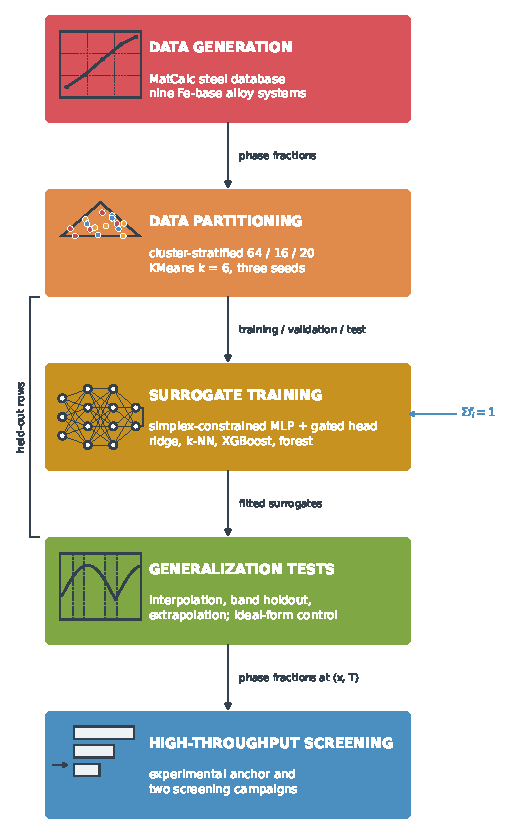
\includegraphics[width=0.88\textwidth]{figures/fig0_workflow}
\caption{Study pipeline. (1) CALPHAD data generation: five Fe-based
ternary subsystems are extracted from the open MatCalc steel database,
probe-driven phase sets fix the target dimensionality, structured sampling
draws 11{,}220 candidate points per system, and a mass-balance gate
accepts 44{,}397 equilibria in total. (2) A cluster-stratified 64/16/20
split feeds a constrained MLP with six output heads (plus two mechanism
probes) and four classical baselines, all fitted under one fixed protocol
and three seeds. (3) Three evaluation protocols --- interpolation,
contiguous interior-band holdout, and strict one-sided extrapolation, the
two spatial ones each with a size-matched random control --- plus two
secondary analyses (ablations and boundary-error analysis, dashed arrows).}
\label{fig:workflow}
\end{figure}

% ======================================================================
\section{Data generation}
\label{sec:data}

\subsection{Thermodynamic description}

The source database is the open MatCalc steel database \texttt{mc\_fe\_v2.062}
\citep{matcalc}, which cannot be parsed by pycalphad \citep{pycalphad} in its
raw form. We parse it with a lenient custom parser, extract the five
three-element subsystems, and apply minimal syntax repairs (reference-element
blocks and malformed function ranges). Both a pruned database (constituents
restricted to the system elements) and an unpruned database are built. Equivalence validation on 100 re-solved points
per system confirms the pruning is bit-for-bit inert: maximum
$|\Delta\Np{\phi}| = 0$ and $|\Delta G_m| = 0$~J/mol for all five systems.
All equilibrium calculations are performed with the open-source CALPHAD
implementation pycalphad \citep{pycalphad} against this database, so the
surrogates emulate this specific solver--database combination; their accuracy
is correspondingly bounded by the database's assessments and the solver's
convergence behaviour.

Eligible phase counts are 28 (Fe--Cr--Ni), 31 (Fe--Cr--Mn), 29 (Fe--Cr--Mo),
25 (Fe--Cr--V), and 29 (Fe--Mn--Ni). Pressure is fixed at 101{,}325~Pa
throughout.

\subsection{Probe-driven phase sets}

Running equilibria with all eligible phases costs ${\sim}2.5$~s per point.
Instead, each system is probed with the full eligible set on 2{,}000 points,
and only phases ever observed active are retained as targets
(Table~\ref{tab:systems}). The probe points are fresh Dirichlet draws
(RNG seed 7), independent of the dataset generated afterwards, so no label
from any train/validation/test row enters the phase-set construction.
Phase-set sufficiency is validated on 300 re-solved points per system
(1{,}500 total): maximum $|\Delta\Np{\phi}| \le 6\times10^{-9}$, zero
violations. The target vector is the full probe-active phase-fraction
vector with no occurrence threshold, so $\sum_k y_k = 1$ holds to the
solver's mass-balance tolerance: $|\sum_k y_k - 1| \le 3.3\times10^{-8}$
across all test rows.

The probe does, however, cover the \emph{entire} sampled domain, including
regions that later become test rows. Phase-set discovery is therefore a
global, transductive preprocessing step: the target dimensionality $K$ is
fixed with knowledge of the whole design space before any predictive split.
This is deliberate --- the surrogate's task is to predict fractions over a
known phase basis, and discovering that basis is part of building the
oracle interface, not part of the predictive task. It is not label
leakage in the ordinary sense (no test label is seen), but it does mean
that a phase active only in an unprobed region would be missed, and that
the reported accuracies are conditional on this globally predefined phase
basis being complete; the experiments do not assess discovery of previously
unseen phases (Section~\ref{sec:discussion}).

\begin{table}[htbp]
\centering
\caption{Systems, probe-active phase counts $K$, and target phases.
``Eligible'' is the number of phases in the full database subset; $K$ is the
number ever observed active in the probe.}
\label{tab:systems}
\small
% Generated by paper/tables.py -- do not edit by hand.
% Table 1: systems, phases, eligibility
\setlength{\tabcolsep}{4pt}
\begin{tabular}{llrrp{6.6cm}}
\toprule
System & $x_2,x_3$ & Eligible & $K$ & Target phases \\
\midrule
Fe--Cr--Ni & Cr, Ni & 28 & 4 & {\raggedright\footnotesize BCC\_A2, FCC\_A1, LIQUID, SIGMA\par} \\
Fe--Cr--Mn & Cr, Mn & 31 & 7 & {\raggedright\footnotesize ALPHA\_MN, BCC\_A2, BETA\_MN, CR3MN5, FCC\_A1, LIQUID, SIGMA\par} \\
Fe--Cr--Mo & Cr, Mo & 29 & 9 & {\raggedright\footnotesize BCC\_A2, CHI\_A12, FCC\_A1, LAVES\_PHASE, LIQUID, MU\_PHASE, MU\_PHASE\_I, R\_PHASE, SIGMA\par} \\
Fe--Cr--V & Cr, V & 25 & 4 & {\raggedright\footnotesize BCC\_A2, FCC\_A1, LIQUID, SIGMA\par} \\
Fe--Mn--Ni & Mn, Ni & 29 & 7 & {\raggedright\footnotesize ALPHA\_MN, BCC\_A2, BETA\_MN, FCC\_A1, LIQUID, MNNI, MNNI2\par} \\
\bottomrule
\end{tabular}

\end{table}

\subsection{Sampling and acceptance}

Design variables per system are $(x_2, x_3, T)$ with $x_{\mathrm{Fe}} =
1 - x_2 - x_3$, temperature uniform in $[700, 2000]$~K. Five deterministic
sampling strategies (RNG seed 42) generate 11{,}220 candidate points:
6{,}000 Fe-weighted uniform draws, 2{,}000 sigma-field-focused draws, 720
grid points on five isothermal slices, 1{,}500 liquidus-zone draws, and
1{,}000 near-pure-Fe draws. A candidate is accepted only if the composition
lies inside the defined sub-simplex and the equilibrium satisfies mass
balance $|\sum_k \Np{k} - 1| < 10^{-6}$. The resulting datasets contain
8{,}880 rows each (8{,}877 for Fe--Cr--Mo, where three points did not
converge). Table~\ref{tab:dataset} summarises the datasets.

The sampling distribution is deliberately structured, not uniform: the
five strategies over-represent the Fe-rich corner, the sigma field, the
liquidus zone, and isothermal grids. This is a design choice --- phase
boundaries and rare-phase regions carry most of the information a
surrogate must learn, and uniform draws would undersample them. The
consequence, which we keep in mind when interpreting results, is that all
reported accuracies are expectations under this distribution; rankings can
shift under a different prior (Section~\ref{sec:discussion}).

\begin{table}[htbp]
\centering
\caption{Dataset composition. ``Box'' is the fraction of rows inside the
stainless-steel box (Fe $\ge$ 0.55, Cr $\le$ 0.30, $x_3 \le$ 0.30).
``Occurrence range'' spans the rarest and most common target phase.}
\label{tab:dataset}
\small
% Generated by paper/tables.py -- do not edit by hand.
% Table 2: dataset composition and closure
\footnotesize
\setlength{\tabcolsep}{4pt}
\renewcommand{\arraystretch}{1.1}
\begin{tabular}{lrrrrl}
\toprule
System & Rows & Box (\%) & $\max|\Sigma y-1|$ & $K$ & Occurrence range (\%) \\
\midrule
Fe--Cr--Ni & 8,880 & 38.0 & $9.8\!\times\!10^{-9}$ & 4 & 11.94--73.6 \\
Fe--Cr--Mn & 8,880 & 38.0 & $1.2\!\times\!10^{-8}$ & 7 & 0.03--57.5 \\
Fe--Cr--Mo & 8,877 & 38.0 & $3.3\!\times\!10^{-8}$ & 9 & 0.10--63.5 \\
Fe--Cr--V & 8,880 & 38.0 & $1.9\!\times\!10^{-8}$ & 4 & 2.04--79.9 \\
Fe--Mn--Ni & 8,880 & 38.0 & $1.9\!\times\!10^{-9}$ & 7 & 0.00--76.0 \\
\bottomrule
\end{tabular}

\end{table}

\begin{figure}[htbp]
\centering
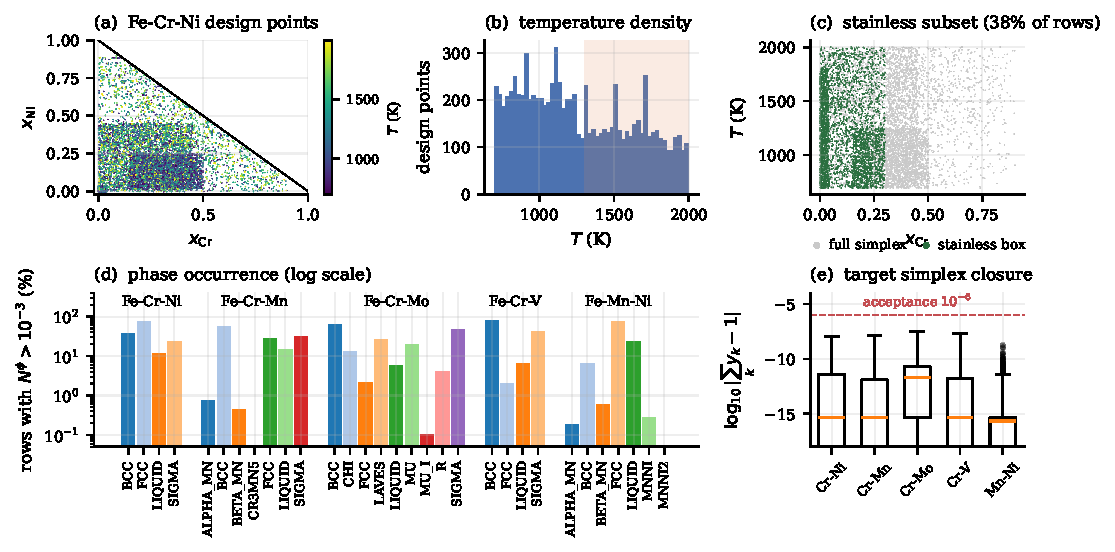
\includegraphics[width=\textwidth]{figures/fig1_dataset}
\caption{Dataset for Fe--Cr--Ni and summary statistics across all five
systems. (a) Design points in the $(x_{\mathrm{Cr}}, x_{\mathrm{Ni}})$
plane coloured by temperature. (b) Temperature density; the shaded band marks
the region above 1300~K where liquid appears. (c) The stainless-steel subset
(green) occupies 38\% of rows. (d) Phase occurrence across all five systems
on a logarithmic scale; rare phases such as MNNI2 (0.00\%) and CR3MN5
(0.03\%) are retained as targets. (e) Simplex closure of the target vectors:
all systems satisfy $|\sum_k y_k - 1| < 10^{-6}$, with the bulk of rows at
$10^{-9}$--$10^{-8}$.}
\label{fig:dataset}
\end{figure}

% ======================================================================
\section{Models and training}
\label{sec:models}

\subsection{Neural-network heads}

The base architecture is a multilayer perceptron with three hidden layers of
192 units (Linear $\to$ LayerNorm $\to$ SiLU $\to$ Dropout 0.1), trained with
AdamW (learning rate $3\times10^{-4}$, weight decay $5\times10^{-4}$, cosine
annealing over 300 epochs, batch size 128, gradient-norm clipping at 1.0,
early stopping on validation MAE with patience 40). The loss is Huber with
$\delta = 0.01$ by default. Inputs are standardised with a
\texttt{StandardScaler} fitted on the training split only. Six output heads
are compared across all five systems (Table~\ref{tab:main}); two further
mechanisms, power normalisation and a sum-to-one loss penalty, are
evaluated on Fe--Cr--Ni only as mechanism probes
(Sections~\ref{sec:ablations}--\ref{sec:negative}).

The \emph{sigmoid} head applies $\sigma(\mathbf{z})$ without normalisation
and serves as the unconstrained control. The \emph{softmax} head applies
$\mathrm{softmax}(\mathbf{z})$. The \emph{sigmoid/$\Sigma$} head computes
$\sigma(\mathbf{z}) / \sum_k \sigma(z_k)$ at train time. The \emph{renorm}
head applies $\sigma(\mathbf{z})$ and then clips to $[0,1]$ and divides by
the row sum as a post-hoc projection. The \emph{sparsemax} head applies the
sparsemax operator \citep{martins2016sparsemax} to $4\mathbf{z}$, producing
exact zeros. The \emph{residue} head predicts $K{-}1$ fractions with
sigmoids and closes the sum algebraically, $\hat y_K = 1 - \sum_{k<K}
\hat y_k$; it enforces the sum-to-one equality by construction but does
\emph{not} intrinsically guarantee non-negativity, so it is not a fully
simplex-valid output (Section~\ref{sec:negative}). The two Fe--Cr--Ni
probes are the \emph{power-norm} head, $\sigma(\mathbf{z})^2 / \sum_k
\sigma(z_k)^2$, and the \emph{penalty} head, $\sigma(\mathbf{z})$ plus
$\lambda(\sum_k \hat y_k - 1)^2$ added to the loss.

We distinguish two properties that the literature often conflates.
\emph{Closure} is the equality $\sum_k \hat y_k = 1$ alone. \emph{Simplex
membership} is Eq.~\eqref{eq:simplex} in full: closure \emph{and}
$\hat y_k \ge 0$ for every $k$. Softmax, sigmoid/$\Sigma$, sparsemax, and
power-norm guarantee both; renorm guarantees both after its projection;
the residue head guarantees closure only.

Non-softmax heads use a per-phase two-layer output block ($192 \to 192 \to 1$)
and a learnable per-phase output scale.

\subsection{Baselines}

Four classical models are fitted one output channel at a time on the raw
targets: ridge regression ($\alpha = 1$), $k$-nearest neighbours ($k = 10$,
distance-weighted), XGBoost \citep{chen2016xgboost} (500 trees, depth 8,
learning rate 0.05, early stopping at 50 rounds), and random forest (500
trees, depth 20) \citep{breiman2001random}. Each is evaluated raw and after
post-hoc renormalisation; the renormalised versions are the physically
admissible ones reported in the main comparison. All hyperparameters ---
neural and classical --- are fixed for the study: the comparison is intended
to isolate output-constraint and model-family behaviour under a fixed,
reproducible protocol rather than to identify globally optimal
hyperparameters for any model family.

\subsection{Splitting, seeds, and metrics}

The split is cluster-stratified: KMeans ($k = 6$, seed-dependent
initialisation) on standardised $(x_2, x_3, T)$, with each cluster
contributing 64/16/20 train/validation/test by seed-dependent permutation.
Six clusters give a coarse stratification of the three-dimensional design
space while keeping each cluster large enough ($\sim$1{,}500 rows) for a
stable within-cluster permutation. The validation partition is used only
for early stopping and XGBoost's stopping criterion; the test partition is
never touched during training or model selection, so all reported test
metrics are computed on data that played no role in fitting. Three
seeds (42, 123, 2024) control all stochastic stages; every reported number is
mean $\pm$ standard deviation over seeds, a measure of seed-to-seed training
stochasticity only, not a full uncertainty quantification (which would
additionally cover sampling, architecture, phase-set, and database
uncertainty). The test set is capped at 4{,}000
rows.

The primary metric is the mean absolute error averaged over phases,
\begin{equation}
    \mathrm{MAE} = \frac{1}{K} \sum_{k=1}^{K}
    \frac{1}{n} \sum_{i=1}^{n} |\hat y_{ik} - y_{ik}|.
    \label{eq:mae}
\end{equation}
Simplex closure is measured as $\mathrm{mean}\,|\sum_k \hat y_k - 1|$.
Phase-presence detection is assessed by per-phase $F_1$ and balanced accuracy
(active if $\Np{k} > 10^{-3}$), averaged over phases. A phase with no
active row in a given test set (MNNI2, with zero active rows in the whole
Fe--Mn--Ni dataset) has an undefined $F_1$; we score it as $F_1 = 0$ for
every model, which keeps the phase in the average without favouring any
model. The $10^{-3}$
threshold is a practical choice: it sits two orders of magnitude below the
smallest non-trivial fraction a lever-rule calculation would report, and
above the solver's numerical noise floor ($\sim 10^{-8}$). Detection
conclusions are checked against this choice in
Section~\ref{sec:detection}, where the same metrics at $10^{-4}$ and
$10^{-2}$ leave the qualitative picture unchanged. An entropy-weighted MAE
weights rows by $1 + H(\mathbf{y})/H_{\max}$ with $H_{\max} = \ln K$,
up-weighting multi-phase coexistence states, where several non-zero
fractions must be predicted simultaneously; it is an auxiliary reporting
metric, not a theoretically privileged loss.

% ======================================================================
\section{Main accuracy}
\label{sec:results}

Table~\ref{tab:main} reports the test MAE for all heads and baselines across
the five systems. Figure~\ref{fig:heads} visualises the comparison.

\begin{table}[htbp]
\centering
\caption{Test MAE (mean over three seeds; uncertainty in units of the last
digit). Best per system in bold. Heads are grouped by whether they satisfy
Eq.~\eqref{eq:simplex} structurally (on-simplex: softmax,
sigmoid/$\Sigma$, sparsemax, renorm after its projection, power-norm), fail
to satisfy it (off-simplex: the unconstrained sigmoid and the closure-only
residue head), or are baselines (shown after post-hoc renormalisation). Six
heads are compared across all five systems; the power-normalisation head
($\dagger$) was evaluated on Fe--Cr--Ni only.}
\label{tab:main}
\small
% Generated by paper/tables.py -- do not edit by hand.
% Table 3: main comparison, test MAE
\scriptsize
\setlength{\tabcolsep}{3pt}
\renewcommand{\arraystretch}{1.1}
\begin{tabular}{llccccc}
\toprule
 & Model & Fe--Cr--Ni & Fe--Cr--Mn & Fe--Cr--Mo & Fe--Cr--V & Fe--Mn--Ni \\
\midrule
\multirow{2}{*}{\rotatebox{90}{\tiny off-simplex}} & sigmoid (unconstrained) & 0.0232\,(10) & 0.0163\,(1) & 0.0184\,(5) & 0.0287\,(4) & 0.0231\,(13) \\
 & residue, $y_d = 1-\Sigma$ & 0.0229\,(3) & 0.0186\,(4) & 0.0182\,(5) & 0.0254\,(3) & 0.0210\,(12) \\
\multirow{5}{*}{\rotatebox{90}{\tiny on-simplex}} & sparsemax & 0.0444\,(229) & 0.0212\,(177) & 0.0573\,(427) & 0.0304\,(161) & 0.0375\,(295) \\
 & softmax & 0.0130\,(3) & 0.0088\,(11) & 0.0148\,(1) & 0.0167\,(2) & 0.0145\,(15) \\
 & sigmoid/$\Sigma$ (train-time) & 0.0112\,(10) & \textbf{0.0074\,(2)} & 0.0126\,(2) & 0.0153\,(4) & 0.0145\,(20) \\
 & sigmoid + renorm (post hoc) & \textbf{0.0106\,(6)} & 0.0081\,(4) & 0.0159\,(3) & 0.0149\,(4) & 0.0140\,(13) \\
 & power-normalisation$^{\dagger}$ & 0.0123\,(14) & --- & --- & --- & --- \\
\midrule
\multirow{4}{*}{\rotatebox{90}{\tiny baselines}} & ridge & 0.2053\,(9) & 0.1399\,(5) & 0.1244\,(6) & 0.1940\,(8) & 0.0769\,(5) \\
 & $k$-NN, $k=10$ & 0.0256\,(6) & 0.0171\,(5) & 0.0151\,(6) & 0.0222\,(5) & 0.0091\,(6) \\
 & XGBoost & 0.0212\,(6) & 0.0154\,(8) & 0.0137\,(2) & 0.0179\,(3) & 0.0081\,(3) \\
 & random forest & 0.0180\,(2) & 0.0133\,(5) & \textbf{0.0123\,(2)} & \textbf{0.0137\,(4)} & \textbf{0.0058\,(3)} \\
\midrule
\multicolumn{7}{l}{\scriptsize $^{\dagger}$Evaluated on Fe--Cr--Ni only (mechanism probe; see Section~\ref{sec:negative}).} \\
\bottomrule
\end{tabular}

\end{table}

\begin{figure}[htbp]
\centering
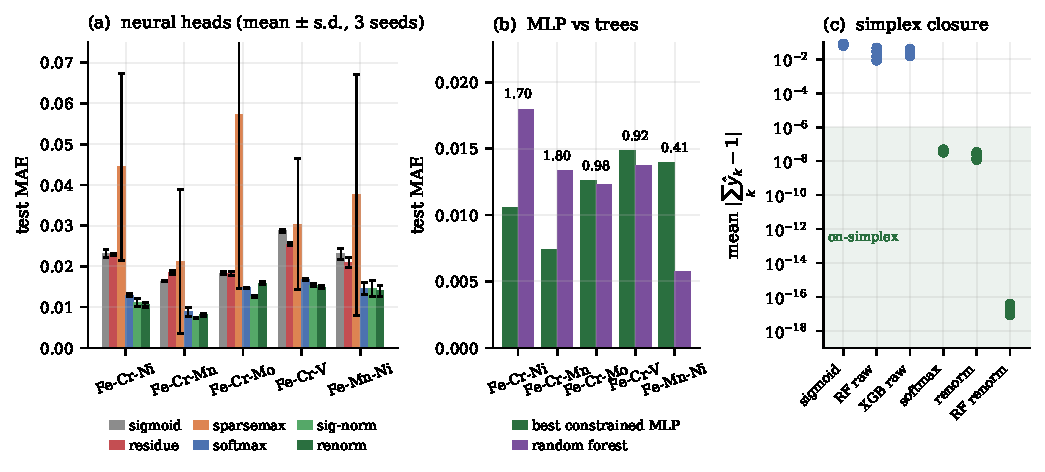
\includegraphics[width=\textwidth]{figures/fig2_heads}
\caption{Main comparison. (a) Test MAE for the six neural heads across all
five systems (mean $\pm$ s.d., three seeds). (b) Best constrained MLP versus
random forest; the annotation gives the RF/MLP ratio. (c) Simplex closure:
constrained heads and renormalised baselines sit at or below $10^{-8}$;
unconstrained outputs violate closure by $10^{-2}$--$10^{-1}$.}
\label{fig:heads}
\end{figure}

\paragraph{Constrained MLPs lead on smooth-coexistence systems.}
On Fe--Cr--Ni the renorm head achieves $0.0106 \pm 0.0006$ against
$0.0180 \pm 0.0002$ for the random forest --- a 41\% reduction, roughly
$12\times$ the seed standard deviation. On Fe--Cr--Mn the sigmoid/$\Sigma$
head achieves $0.0074 \pm 0.0002$ against $0.0133 \pm 0.0005$ for the forest.
Both systems feature extended smooth two- and three-phase coexistence fields
(sigma with BCC/FCC in Fe--Cr--Ni; the Laves, mu, R and chi intermetallic
family in Fe--Cr--Mo), which favour the smooth function class of the MLP.

\paragraph{Trees win where boundaries are sharp.}
On Fe--Cr--V the forest achieves $0.0137 \pm 0.0004$ against
$0.0149 \pm 0.0004$ for the best MLP; on Fe--Mn--Ni the gap is larger:
$0.0058 \pm 0.0003$ for the forest against $0.0140 \pm 0.0013$ for the
best MLP. Both systems are dominated by sharp, essentially binary phase
boundaries (BCC$\leftrightarrow$SIGMA/\allowbreak FCC in Fe--Cr--V;
FCC$\leftrightarrow$LIQUID in Fe--Mn--Ni) with rare phases.
Axis-aligned tree splits can represent such sharp transitions efficiently.

\paragraph{Fe--Cr--Mo is a statistical tie.}
The random forest ($0.0123 \pm 0.0002$) and sigmoid/$\Sigma$
($0.0126 \pm 0.0002$) differ by 0.0003, comparable to the seed standard
deviation. The system's nine-phase target vector, with its intermetallic
family, provides enough smooth structure for the MLP to compete but enough
sharp boundaries for the forest to match it.

\paragraph{Paired bootstrap confirms the ranking and the ties.}
Three seeds give limited statistical power, so we paired the two models'
per-row errors on the identical test rows and resampled with replacement
(10{,}000 paired bootstrap resamples of the test rows, three seeds pooled;
Table~\ref{tab:bootstrap}). The
95\% confidence interval of the mean-MAE difference excludes zero in favour
of the MLP on Fe--Cr--Ni and Fe--Cr--Mn and in favour of the random forest
on Fe--Mn--Ni, while it includes zero on Fe--Cr--Mo and Fe--Cr--V: the two
near-ties claimed above are genuine ties, not under-powered comparisons.

\begin{table}[htbp]
\centering
\caption{Paired bootstrap comparison of the best constrained MLP head and
the random forest on the interpolation test set. $\overline{\Delta}$MAE is
the mean per-row MAE difference (MLP $-$ RF); a negative value favours the
MLP. CI: 95\% bootstrap confidence interval (10{,}000 paired bootstrap
resamples of the test rows, three seeds pooled).}
\label{tab:bootstrap}
\small
% Generated by paper/tables.py -- do not edit by hand.
% Table 10: paired bootstrap, best constrained MLP vs random forest
\footnotesize
\setlength{\tabcolsep}{4pt}
\begin{tabular}{llccc}
\toprule
System & Best MLP head & $\overline{\Delta}$MAE & 95\% CI & verdict \\
\midrule
Fe--Cr--Ni & renorm & $-0.00737$ & $[-0.00850,\,-0.00627]$ & MLP better \\
Fe--Cr--Mn & sig-norm & $-0.00593$ & $[-0.00670,\,-0.00514]$ & MLP better \\
Fe--Cr--Mo & sig-norm & $+0.00027$ & $[-0.00054,\,+0.00109]$ & tie \\
Fe--Cr--V & renorm & $+0.00115$ & $[-0.00071,\,+0.00303]$ & tie \\
Fe--Mn--Ni & renorm & $+0.00821$ & $[+0.00678,\,+0.00970]$ & RF better \\
\bottomrule
\end{tabular}

\end{table}

\paragraph{Post-hoc renormalisation did not hurt accuracy in any of the
five systems tested.}
All four evaluated baselines improve or remain unchanged under
renormalisation, by $0.0000$--$0.0004$ for the
random forest and $k$-NN, $0.0007$--$0.0020$ for XGBoost, and
$0.0066$--$0.0163$ for ridge. The larger the simplex violation, the more the
projection recovers.

% ======================================================================
\section{Simplex closure}
\label{sec:closure}

Table~\ref{tab:closure} reports the mean closure violation. All
structurally constrained heads satisfy $\sum_k \hat y_k = 1$ to
$\le 5\times10^{-8}$ --- float32 round-off over $K$ terms. The unconstrained
sigmoid violates closure by 6--8\% on average. Raw tree outputs violate it by
0.9--4.7\%. Post-hoc renormalisation repairs all evaluated models to machine precision
(${\sim}10^{-17}$).

Closure, however, is only half of Eq.~\eqref{eq:simplex}. The residue head
closes the sum by construction yet still emits negative fractions on
0.0--1.2\% of cells depending on the system (Section~\ref{sec:negative}),
so it is closure-valid but not simplex-valid. All other constrained heads
and the renormalised baselines satisfy both conditions.

\begin{table}[htbp]
\centering
\caption{Mean closure violation $\mathrm{mean}\,|\sum_k \hat y_k - 1|$ on
the test set (mean over three seeds). Structural constraints achieve
closure to float32 precision; post-hoc renormalisation achieves machine
precision; unconstrained outputs violate closure by orders of magnitude.
Closure is the equality constraint only; see the text for
non-negativity.}
\label{tab:closure}
\small
% Generated by paper/tables.py -- do not edit by hand.
% Table 4: simplex closure
\footnotesize
\setlength{\tabcolsep}{4pt}
\renewcommand{\arraystretch}{1.1}
\begin{tabular}{llccccc}
\toprule
Closure & Model & Fe--Cr--Ni & Fe--Cr--Mn & Fe--Cr--Mo & Fe--Cr--V & Fe--Mn--Ni \\
\midrule
none & sigmoid & $6.2\!\times\!10^{-2}$ & $8.1\!\times\!10^{-2}$ & $8.1\!\times\!10^{-2}$ & $6.3\!\times\!10^{-2}$ & $7.4\!\times\!10^{-2}$ \\
 & random forest, raw & $2.8\!\times\!10^{-2}$ & $2.9\!\times\!10^{-2}$ & $4.7\!\times\!10^{-2}$ & $1.5\!\times\!10^{-2}$ & $8.7\!\times\!10^{-3}$ \\
 & XGBoost, raw & $2.8\!\times\!10^{-2}$ & $3.3\!\times\!10^{-2}$ & $4.1\!\times\!10^{-2}$ & $2.1\!\times\!10^{-2}$ & $1.6\!\times\!10^{-2}$ \\
\addlinespace
structural & softmax & $3.3\!\times\!10^{-8}$ & $4.8\!\times\!10^{-8}$ & $4.4\!\times\!10^{-8}$ & $3.4\!\times\!10^{-8}$ & $4.5\!\times\!10^{-8}$ \\
 & sigmoid/$\Sigma$ & $1.7\!\times\!10^{-8}$ & $2.7\!\times\!10^{-8}$ & $3.3\!\times\!10^{-8}$ & $1.6\!\times\!10^{-8}$ & $3.1\!\times\!10^{-8}$ \\
 & sparsemax & $1.7\!\times\!10^{-8}$ & $1.8\!\times\!10^{-8}$ & $5.0\!\times\!10^{-8}$ & $1.0\!\times\!10^{-8}$ & $4.0\!\times\!10^{-10}$ \\
 & residue & $9.2\!\times\!10^{-9}$ & $1.9\!\times\!10^{-8}$ & $1.8\!\times\!10^{-8}$ & $6.5\!\times\!10^{-9}$ & $1.8\!\times\!10^{-8}$ \\
\addlinespace
post hoc & sigmoid + renorm & $1.5\!\times\!10^{-8}$ & $2.5\!\times\!10^{-8}$ & $2.5\!\times\!10^{-8}$ & $1.2\!\times\!10^{-8}$ & $3.3\!\times\!10^{-8}$ \\
 & random forest + renorm & $2.3\!\times\!10^{-17}$ & $2.0\!\times\!10^{-17}$ & $3.8\!\times\!10^{-17}$ & $1.5\!\times\!10^{-17}$ & $8.9\!\times\!10^{-18}$ \\
\bottomrule
\end{tabular}

\end{table}

The closure result has a practical consequence: a surrogate whose output
violates Eq.~\eqref{eq:simplex} cannot be used directly in any downstream
calculation that assumes a valid phase assemblage --- lever-rule property
averaging, for instance, or a subsequent kinetic simulation. The constrained
heads and post-hoc renormalisation both produce admissible outputs; the
former do so without a separate projection step.

% ======================================================================
\section{Regression versus detection}
\label{sec:detection}

Table~\ref{tab:detection} and Figure~\ref{fig:perphase} reveal a gap between
regression accuracy and phase-presence detection. The two are distinct
tasks: the model that best estimates continuous phase fractions need not be
the model that best identifies phase presence, and the model with the lowest
MAE is not always the best detector.

\begin{table}[htbp]
\centering
\caption{Regression versus detection. For each system the best constrained
MLP head and the random forest are compared on MAE, mean $F_1$, balanced
accuracy, and entropy-weighted MAE. The MLP is the better regressor on two
systems (with a near-tie on Fe--Cr--Mo) but the worse detector on three.}
\label{tab:detection}
\small
% Generated by paper/tables.py -- do not edit by hand.
% Table 5: regression vs detection
\footnotesize
\setlength{\tabcolsep}{4pt}
\renewcommand{\arraystretch}{1.1}
\begin{tabular}{llcccc}
\toprule
System & Model & MAE & $F_1$ & bal.\ acc. & entropy-w.\ MAE \\
\midrule
Fe--Cr--Ni & MLP renorm & 0.0106 & 0.927 & 0.939 & 0.0137 \\
 & random forest & 0.0180 & 0.846 & 0.887 & 0.0218 \\
\addlinespace
Fe--Cr--Mn & MLP sig-norm & 0.0074 & 0.527 & 0.752 & 0.0089 \\
 & random forest & 0.0133 & 0.592 & 0.850 & 0.0150 \\
\addlinespace
Fe--Cr--Mo & MLP sig-norm & 0.0126 & 0.643 & 0.827 & 0.0149 \\
 & random forest & 0.0123 & 0.629 & 0.858 & 0.0147 \\
\addlinespace
Fe--Cr--V & MLP renorm & 0.0149 & 0.718 & 0.822 & 0.0167 \\
 & random forest & 0.0137 & 0.785 & 0.893 & 0.0158 \\
\addlinespace
Fe--Mn--Ni & MLP renorm & 0.0140 & 0.312 & 0.643 & 0.0158 \\
 & random forest & 0.0058 & 0.504 & 0.884 & 0.0063 \\
\bottomrule
\end{tabular}

\end{table}

\begin{figure}[htbp]
\centering
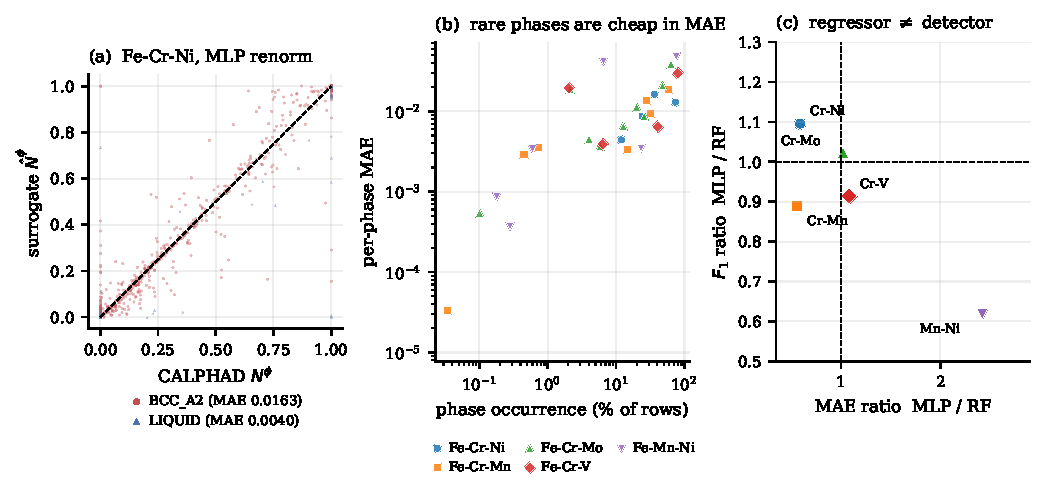
\includegraphics[width=\textwidth]{figures/fig4_perphase}
\caption{Per-phase accuracy and the regressor--detector gap. (a) Parity plot
for the hardest and easiest phase of Fe--Cr--Ni under the renorm head.
(b) Per-phase MAE versus phase occurrence across all five systems: rare
phases are cheap in aggregate MAE because the dominant zero-fraction rows
contribute little error. (c) MAE ratio versus $F_1$ ratio (MLP over random
forest): systems below the diagonal have an MLP that regresses better but
detects worse.}
\label{fig:perphase}
\end{figure}

\paragraph{Rare phases are cheap in aggregate MAE and hard to detect.}
Aggregate MAE can underweight rare phases because the dominant zero-fraction
rows contribute almost no error: a phase present in 0.1\% of rows
contributes little to the average whether the model predicts it correctly
or not. Low MAE on such a phase is therefore not evidence that the model
represents it; it is an artefact of the averaging. Detecting its presence
--- the metallurgically important question --- requires the model to
distinguish a small positive signal from noise, which is what the
presence metrics measure. On Fe--Mn--Ni the MLP predicts MNNI, MNNI2, and
ALPHA\_MN as absent ($F_1 = 0$ for all three) while the random forest
resolves two of them.

\paragraph{The gap is stable across presence thresholds.}
The presence threshold $\Np{k} > 10^{-3}$ is a modelling decision, so we
recomputed $F_1$ at $10^{-4}$ and $10^{-2}$ from the stored predictions
(Table~\ref{tab:threshold}). Absolute $F_1$ values move --- stricter
thresholds make detection harder --- but the ordering does not on four of
five systems: the random forest remains the better detector on Fe--Cr--Mn,
Fe--Cr--V, and Fe--Mn--Ni at all three thresholds, and the MLP on Fe--Cr--Ni.
On Fe--Cr--Mo the better detector flips with the threshold, consistent
with that system's overall tie. The regressor--detector gap is not an
artefact of the threshold choice.

\begin{table}[htbp]
\centering
\caption{Sensitivity of phase-presence detection to the presence threshold.
Mean $F_1$ (three seeds; uncertainty in units of the last digit) for the
best constrained MLP head and the random forest at thresholds $10^{-4}$,
$10^{-3}$ (main-study default), and $10^{-2}$.}
\label{tab:threshold}
\small
% Generated by paper/tables.py -- do not edit by hand.
% Table 9: threshold sensitivity of phase-presence detection
\footnotesize
\setlength{\tabcolsep}{4pt}
\renewcommand{\arraystretch}{1.1}
\begin{tabular}{llccc}
\toprule
System & Model & $F_1$ at $10^{-4}$ & $F_1$ at $10^{-3}$ & $F_1$ at $10^{-2}$ \\
\midrule
Fe--Cr--Ni & best MLP (renorm) & 0.870\,(6) & 0.927\,(4) & 0.962\,(3) \\
 & random forest & 0.815\,(6) & 0.846\,(6) & 0.911\,(2) \\
\addlinespace
Fe--Cr--Mn & best MLP (sig-norm) & 0.489\,(6) & 0.527\,(2) & 0.550\,(2) \\
 & random forest & 0.571\,(20) & 0.592\,(18) & 0.672\,(19) \\
\addlinespace
Fe--Cr--Mo & best MLP (sig-norm) & 0.562\,(13) & 0.643\,(2) & 0.710\,(3) \\
 & random forest & 0.590\,(2) & 0.629\,(3) & 0.727\,(4) \\
\addlinespace
Fe--Cr--V & best MLP (renorm) & 0.671\,(35) & 0.718\,(1) & 0.731\,(1) \\
 & random forest & 0.767\,(6) & 0.785\,(9) & 0.870\,(6) \\
\addlinespace
Fe--Mn--Ni & best MLP (renorm) & 0.306\,(5) & 0.312\,(4) & 0.314\,(4) \\
 & random forest & 0.470\,(0) & 0.504\,(1) & 0.603\,(21) \\
\bottomrule
\end{tabular}

\end{table}

\paragraph{Detection degrades faster than regression under shift.}
This gap widens under distribution shift. On the held-out temperature band of
Fe--Cr--Ni, the MLP's mean $F_1$ drops from 0.93 to 0.64 while its MAE rises
only from 0.010 to 0.013 (Section~\ref{sec:extrapolation}). Phase-presence
detection is the first casualty of leaving the training distribution.

% ======================================================================
\section{Spatial generalisation: contiguous holdout and strict
extrapolation}
\label{sec:extrapolation}

\subsection{Two protocols, each with a random control}

The cluster-stratified split of Section~\ref{sec:models} is an interpolation
test. We add two spatial protocols; in both the model is retrained from
scratch (same protocol, three seeds, four models, five systems).

\emph{Contiguous interior-band holdout.} Two blocks are removed from
training and used as the test set: a temperature band $T \in [1200,
1400]$~K (1{,}275 rows) and a composition band $x_2 \in [0.25, 0.35]$
(1{,}676 rows). Because training rows remain on both sides of each band,
this is a missing-region generalisation test, not strict extrapolation. We
verified this geometrically: a Delaunay triangulation of the remaining
training points in scaled $(x_2, x_3, T)$ coordinates shows that
99.3--99.4\% of the held-out band rows lie \emph{inside} the convex hull of
the training set in all five systems. The held-out region is a hole in the
sampling, not an out-of-support region.

\emph{Strict one-sided out-of-range extrapolation.} Training keeps only the
near side of one coordinate and the test set is the far side, with the
interior gap in neither split: train $x_2 \le 0.25$, test $x_2 > 0.35$
(2{,}679 test rows on Fe--Cr--Ni); and train $T \le 1200$~K, test $T >
1400$~K (3{,}219 test rows). Every test point now lies outside the training
range of the extrapolated coordinate by construction. This is strict
out-of-range extrapolation \emph{along one coordinate at a time}; it does
not imply that the whole multidimensional chemical space of the test rows
is unseen, since the other coordinates remain inside their training ranges.

The random controls are the key methodological element of both protocols.
Removing a region also removes training data, so a bare
region-versus-interpolation comparison cannot separate ``cannot generalise
there'' from ``had less to learn from''. Each block therefore has a
size-matched control: the same number of rows removed from training at
random, with an equal-size random test set. Any degradation beyond the
control is spatial. Table~\ref{tab:holdout} reports the band results and
Table~\ref{tab:extrap} the extrapolation results;
Figure~\ref{fig:ablation} panel (a) shows the band penalty ratios and
Figure~\ref{fig:extrap} the extrapolation ones.

\begin{table}[htbp]
\centering
\caption{Contiguous interior-band holdout. Top: test MAE on the random
control, the held-out temperature band, and the held-out composition band
(mean over three seeds; uncertainty in units of the last digit). Bottom:
penalty ratios (band MAE / control MAE) for the temperature and composition
bands. A ratio above 1 indicates a spatial penalty beyond the data-volume
effect.}
\label{tab:holdout}
\small
% Generated by paper/tables.py -- do not edit by hand.
% Table 6: contiguous interior-band holdout
\scriptsize
\setlength{\tabcolsep}{3pt}
\resizebox{\textwidth}{!}{
\begin{tabular}{llccccc}
\toprule
Held-out region & Model & Fe--Cr--Ni & Fe--Cr--Mn & Fe--Cr--Mo & Fe--Cr--V & Fe--Mn--Ni \\
\midrule
\multirow{4}{*}{random control} & MLP renorm & 0.0101\,(8) & 0.0083\,(6) & 0.0153\,(5) & 0.0234\,(70) & 0.0122\,(2) \\
 & MLP sigmoid/$\Sigma$ & 0.0107\,(10) & 0.0077\,(6) & 0.0125\,(7) & 0.0146\,(13) & 0.0123\,(1) \\
 & random forest & 0.0198\,(11) & 0.0142\,(5) & 0.0140\,(11) & 0.0155\,(12) & 0.0058\,(4) \\
 & XGBoost & 0.0237\,(9) & 0.0167\,(6) & 0.0152\,(11) & 0.0194\,(7) & 0.0084\,(1) \\
\addlinespace
\multirow{4}{*}{$T \in [1200,1400]$\,K} & MLP renorm & 0.0132\,(9) & 0.0079\,(4) & 0.0266\,(4) & 0.0358\,(3) & 0.0022\,(0) \\
 & MLP sigmoid/$\Sigma$ & 0.0144\,(32) & 0.0077\,(0) & 0.0265\,(4) & 0.0372\,(12) & 0.0024\,(2) \\
 & random forest & 0.0258\,(10) & 0.0123\,(2) & 0.0309\,(12) & 0.0762\,(97) & 0.0090\,(6) \\
 & XGBoost & 0.0408\,(17) & 0.0203\,(16) & 0.0348\,(17) & 0.0823\,(77) & 0.0167\,(7) \\
\addlinespace
\multirow{4}{*}{$x_2 \in [0.25,0.35]$} & MLP renorm & 0.0162\,(7) & 0.0071\,(0) & 0.0155\,(5) & 0.0111\,(52) & 0.0005\,(0) \\
 & MLP sigmoid/$\Sigma$ & 0.0163\,(6) & 0.0071\,(3) & 0.0144\,(7) & 0.0075\,(15) & 0.0010\,(5) \\
 & random forest & 0.0615\,(73) & 0.0223\,(6) & 0.0259\,(9) & 0.0288\,(5) & 0.0043\,(1) \\
 & XGBoost & 0.0530\,(22) & 0.0250\,(11) & 0.0324\,(3) & 0.0368\,(27) & 0.0063\,(7) \\
\midrule
penalty $T$/$x_2$ & MLP renorm & 1.31 / 1.61 & 0.95 / 0.85 & 1.74 / 1.01 & 1.53 / 0.48 & 0.18 / 0.04 \\
 & MLP sigmoid/$\Sigma$ & 1.34 / 1.52 & 1.00 / 0.92 & 2.12 / 1.16 & 2.55 / 0.52 & 0.20 / 0.08 \\
 & random forest & 1.31 / 3.11 & 0.86 / 1.57 & 2.21 / 1.85 & 4.92 / 1.86 & 1.54 / 0.73 \\
 & XGBoost & 1.72 / 2.24 & 1.21 / 1.49 & 2.29 / 2.13 & 4.24 / 1.89 & 2.00 / 0.75 \\
\bottomrule
\end{tabular}}

\end{table}

\begin{table}[htbp]
\centering
\caption{Strict one-sided out-of-range extrapolation: training keeps only
the near side of one coordinate, the test set is the far side, and the
interior gap is in neither split. Composition extrapolation: train $x_2 \le
0.25$, test $x_2 > 0.35$; temperature extrapolation: train $T \le 1200$~K,
test $T > 1400$~K. Top: test MAE on the far side against size-matched random
controls (mean over three seeds; uncertainty in units of the last digit).
Bottom: penalty ratios (far-side MAE / matched-control MAE) for
composition and temperature extrapolation.}
\label{tab:extrap}
\small
% Generated by paper/tables.py -- do not edit by hand.
% Table 7: strict out-of-range extrapolation
\footnotesize
\setlength{\tabcolsep}{4pt}
\renewcommand{\arraystretch}{1.1}
\resizebox{\textwidth}{!}{
\begin{tabular}{llccccc}
\toprule
Region & Model & Fe--Cr--Ni & Fe--Cr--Mn & Fe--Cr--Mo & Fe--Cr--V & Fe--Mn--Ni \\
\midrule
\multirow{4}{*}{random control ($x_2$-matched)} & MLP renorm & 0.0123\,(3) & 0.0094\,(2) & 0.0181\,(5) & 0.0242\,(73) & 0.0135\,(6) \\
 & MLP sigmoid/$\Sigma$ & 0.0128\,(16) & 0.0092\,(3) & 0.0144\,(5) & 0.0163\,(13) & 0.0146\,(10) \\
 & random forest & 0.0236\,(7) & 0.0168\,(1) & 0.0167\,(6) & 0.0191\,(11) & 0.0084\,(2) \\
 & XGBoost & 0.0283\,(14) & 0.0202\,(7) & 0.0184\,(5) & 0.0235\,(16) & 0.0118\,(2) \\
\addlinespace
\multirow{4}{*}{$x_2$ extrapolation} & MLP renorm & 0.1721\,(77) & 0.0458\,(17) & 0.0668\,(26) & 0.0464\,(66) & 0.0143\,(25) \\
 & MLP sigmoid/$\Sigma$ & 0.1709\,(65) & 0.0526\,(28) & 0.0689\,(8) & 0.0478\,(60) & 0.0129\,(8) \\
 & random forest & 0.2152\,(9) & 0.0788\,(5) & 0.1052\,(22) & 0.0761\,(50) & 0.0279\,(6) \\
 & XGBoost & 0.2267\,(28) & 0.0860\,(47) & 0.1082\,(12) & 0.1015\,(38) & 0.0329\,(3) \\
\addlinespace
\multirow{4}{*}{random control ($T$-matched)} & MLP renorm & 0.0127\,(2) & 0.0100\,(2) & 0.0187\,(8) & 0.0277\,(4) & 0.0142\,(5) \\
 & MLP sigmoid/$\Sigma$ & 0.0142\,(12) & 0.0102\,(3) & 0.0153\,(4) & 0.0158\,(8) & 0.0151\,(4) \\
 & random forest & 0.0245\,(10) & 0.0178\,(5) & 0.0173\,(6) & 0.0194\,(17) & 0.0080\,(3) \\
 & XGBoost & 0.0285\,(14) & 0.0214\,(3) & 0.0191\,(5) & 0.0243\,(18) & 0.0111\,(1) \\
\addlinespace
\multirow{4}{*}{$T$ extrapolation} & MLP renorm & 0.2227\,(66) & 0.1262\,(41) & 0.0823\,(27) & 0.0994\,(6) & 0.1823\,(0) \\
 & MLP sigmoid/$\Sigma$ & 0.2241\,(96) & 0.1266\,(48) & 0.0796\,(19) & 0.0991\,(11) & 0.1822\,(0) \\
 & random forest & 0.2346\,(4) & 0.1524\,(13) & 0.1073\,(8) & 0.1937\,(10) & 0.1834\,(1) \\
 & XGBoost & 0.2327\,(6) & 0.1536\,(16) & 0.1054\,(5) & 0.1972\,(20) & 0.1841\,(2) \\
\midrule
penalty $x_2$/$T$ & MLP renorm & 13.98 / 17.60 & 4.89 / 12.57 & 3.69 / 4.40 & 1.92 / 3.59 & 1.06 / 12.85 \\
 & MLP sigmoid/$\Sigma$ & 13.36 / 15.78 & 5.74 / 12.46 & 4.78 / 5.19 & 2.93 / 6.25 & 0.88 / 12.05 \\
 & random forest & 9.12 / 9.56 & 4.69 / 8.55 & 6.29 / 6.21 & 3.99 / 9.97 & 3.30 / 22.84 \\
 & XGBoost & 8.02 / 8.16 & 4.25 / 7.19 & 5.87 / 5.51 & 4.31 / 8.11 & 2.79 / 16.64 \\
\bottomrule
\end{tabular}}

\end{table}

\begin{figure}[htbp]
\centering
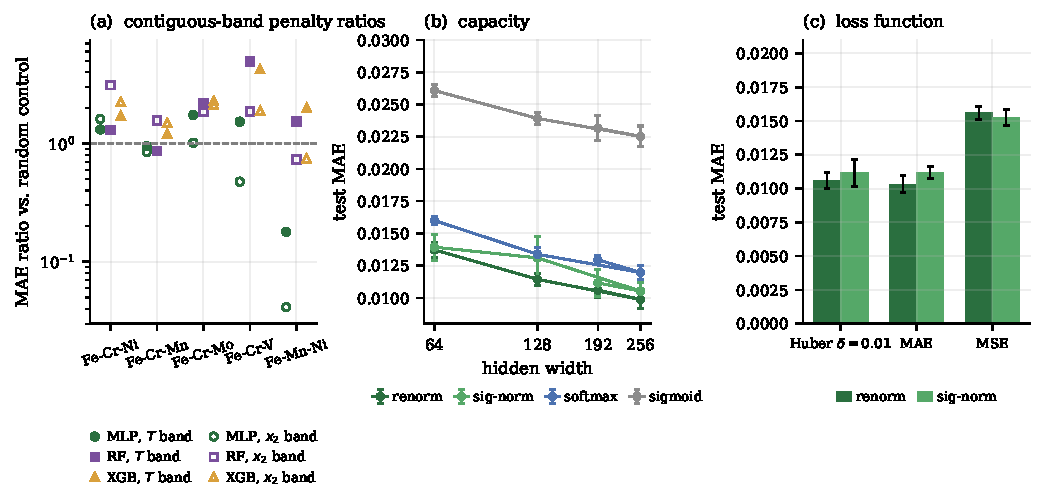
\includegraphics[width=\textwidth]{figures/fig5_ablation}
\caption{(a) Contiguous-band penalty ratios (band MAE / random-control MAE)
across all five systems for the MLP, random forest, and XGBoost. Filled
markers: temperature band; open markers: composition band. The dashed line
at 1.0 marks the random control. (b) Effect of hidden-layer width on test
MAE for four heads on Fe--Cr--Ni. (c) Effect of the loss function on test
MAE for the renorm and sigmoid/$\Sigma$ heads.}
\label{fig:ablation}
\end{figure}

\begin{figure}[htbp]
\centering
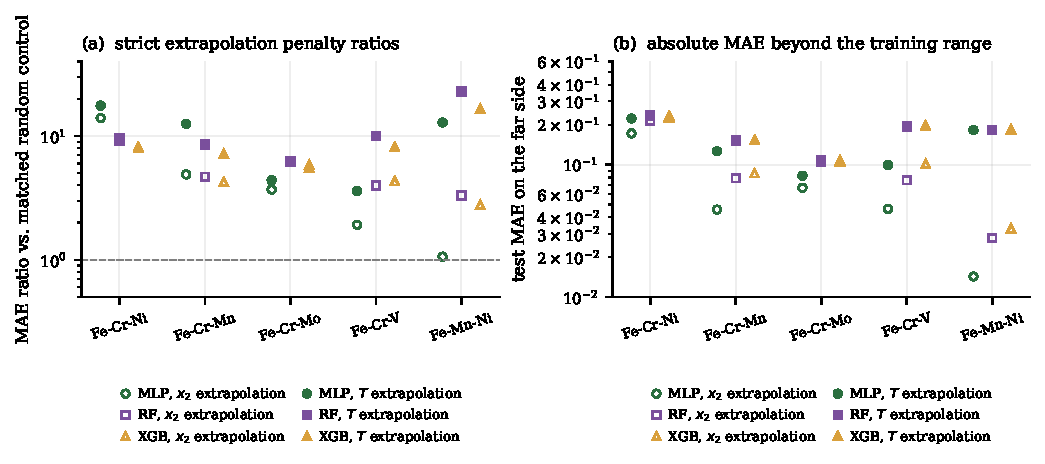
\includegraphics[width=\textwidth]{figures/fig7_extrap}
\caption{Strict one-sided out-of-range extrapolation. (a) Penalty ratios
(far-side MAE / matched random-control MAE) for composition extrapolation
(train $x_2 \le 0.25$, test $x_2 > 0.35$; open markers) and temperature
extrapolation (train $T \le 1200$~K, test $T > 1400$~K; filled markers).
(b) Absolute test MAE on the far side. All evaluated model families degrade
sharply beyond the training range of the extrapolated coordinate; the
constrained MLP achieves the lowest absolute error.}
\label{fig:extrap}
\end{figure}

\subsection{Findings: contiguous interior-band holdout}

\paragraph{The temperature-band penalty is largely a data effect.}
On Fe--Cr--Ni the MLP and the random forest pay the \emph{same} $1.31\times$
penalty once the random control is used as the reference. Comparing the
temperature band against the interpolation split instead would have
suggested that trees cannot generalise in temperature; the size-matched
control shows that the temperature band removes 1{,}275 training rows, and
the resulting data loss, not the spatial shift, accounts for most of the
degradation.

\paragraph{The composition band is where model families separate.}
On Fe--Cr--Ni the random forest pays $3.11\times$ on the composition band
against $1.61\times$ for the constrained MLP ($2.24\times$ for XGBoost).
The same ordering holds on Fe--Cr--Mn ($1.57\times$ versus $0.85\times$) and
Fe--Cr--Mo ($1.85\times$ versus $1.01\times$). Since the held-out rows lie
inside the training convex hull, this is not an extrapolation result in the
strict sense; it is a result about graceful degradation under a contiguous
missing region. Tree-based models partition the input space into
piecewise-constant regions, so predictions inside the hole depend on the
learned partition boundaries and on how the forest aggregates across trees;
this can degrade rapidly when the hole spans a phase-boundary shift, while
the MLP's smooth parametrisation degrades more gracefully.

\paragraph{The composition-band ordering is consistent across all
system--seed pairs.}
As a statistical check on the spatial protocol, we applied a two-sided
sign test to the 15 system$\times$seed penalty-ratio pairs. The MLP's
composition-band penalty is lower than the random forest's and lower than
XGBoost's on all 15 pairs ($p = 6.1\times10^{-5}$ for each comparison).
On the temperature band the MLP--forest difference is not significant
(11 of 15 pairs, $p = 0.12$), consistent with the shared
$1.31\times$ penalty, while the MLP--XGBoost difference remains
significant (15 of 15, $p = 6.1\times10^{-5}$).

\paragraph{The penalty is system-dependent, not universal.}
On Fe--Cr--V the random forest degrades $4.92\times$ on the temperature band
--- a phase-boundary-rich region where the forest's local averaging fails
badly. On Fe--Mn--Ni the held-out bands are \emph{easier} than the random
control ($0.04$--$0.73\times$), because the bands sit in the dataset's easy,
liquid-dominated corner. Generalisation difficulty is a property of the
system and the region, not of the model alone.

\paragraph{Detection collapses on the temperature band.}
Mean $F_1$ drops sharply for all four evaluated models on the temperature
band, even where
MAE barely moves. On Fe--Cr--Ni the MLP's $F_1$ falls from 0.93 (control) to
0.64 (temperature band); the random forest's from 0.84 to 0.53. The
phase-presence decision is more sensitive to distribution shift than the
fraction regression.

\subsection{Findings: strict one-sided out-of-range extrapolation}

\paragraph{All evaluated model families degrade sharply beyond the training
range.}
On Fe--Cr--Ni the composition-extrapolation MAE rises to $\sim$0.17 for the
MLP and $\sim$0.22 for the random forest, against $\sim$0.013 on the
matched control --- an order of magnitude. Temperature extrapolation is
similarly severe. No architecture evaluated in this study extrapolates phase
fractions reliably beyond the trained composition or temperature range;
this is the honest headline of the strict protocol.

\paragraph{The constrained MLP reaches the lowest far-side error.}
In absolute terms the constrained MLP's far-side MAE is the lowest of the
three model families on composition extrapolation in all five systems and
on temperature extrapolation in all five (Figure~\ref{fig:extrap},
panel b). Relative to its own matched control the MLP's penalty ratio can
be \emph{higher} than the trees' --- the trees' controls are themselves
degraded, so the ratio is reference-dependent --- and we report the
absolute-error comparison as the cleaner statement. A two-sided sign test
over the 15 system$\times$seed pairs agrees with that caveat: the MLP's
penalty ratio is lower than the trees' on only 9 of 15 pairs
($p = 0.61$), so the ratio comparison is not significant. The ordering matches
the contiguous-band result: smooth parametrisations degrade more
gracefully than leaf averaging when the query leaves the trained region.
The difference is one of degree, not of kind --- graceful degradation is
not reliable extrapolation.

% ======================================================================
\section{Ablations}
\label{sec:ablations}

Table~\ref{tab:ablation} and Figure~\ref{fig:ablation} panels (b) and (c)
report three ablations on Fe--Cr--Ni.

\begin{table}[htbp]
\centering
\caption{Ablations on Fe--Cr--Ni (mean over three seeds; uncertainty in units
of the last digit). Loss function, hidden-layer width, and closure penalty
are varied for the renorm and sigmoid/$\Sigma$ heads.}
\label{tab:ablation}
\small
% Generated by paper/tables.py -- do not edit by hand.
% Table 8: ablations, Fe-Cr-Ni
\footnotesize
\setlength{\tabcolsep}{4pt}
\renewcommand{\arraystretch}{1.1}
\resizebox{\textwidth}{!}{
\begin{tabular}{llcc}
\toprule
Ablation & Setting & renorm & sigmoid/$\Sigma$ \\
\midrule
\multirow{3}{*}{loss}
 & Huber, $\delta=0.01$ (default) & 0.0106\,(6) & 0.0112\,(10) \\
 & MAE & 0.0103\,(6) & 0.0112\,(4) \\
 & MSE & 0.0156\,(5) & 0.0152\,(6) \\
\addlinespace
\multirow{4}{*}{width}
 & $3\times64$ & 0.0137\,(6) & 0.0139\,(10) \\
 & $3\times128$ & 0.0114\,(5) & 0.0131\,(17) \\
 & $3\times192$ (default) & 0.0106\,(6) & 0.0112\,(10) \\
 & $3\times256$ & 0.0099\,(7) & 0.0105\,(7) \\
\addlinespace
\multirow{3}{*}{closure penalty}
 & none & \multicolumn{2}{c}{0.0232\,(10), closure $6.2\!\times\!10^{-2}$} \\
 & $\lambda=1$ & \multicolumn{2}{c}{0.0804\,(51), closure $2.2\!\times\!10^{-3}$} \\
 & $\lambda=10$ & \multicolumn{2}{c}{0.1693\,(228), closure $1.3\!\times\!10^{-3}$} \\
\bottomrule
\end{tabular}}

\end{table}

\paragraph{Huber and MAE losses are equivalent; MSE is worse.}
The Huber loss with $\delta = 0.01$ and the MAE loss give statistically
indistinguishable results ($0.0106$ versus $0.0103$ for renorm). The MSE
loss is 47\% worse ($0.0156$), because rare-phase outliers dominate the
squared error.

\paragraph{Accuracy improves monotonically with width up to 256.}
Widening the hidden layers from 64 to 256 units reduces the renorm MAE from
$0.0137$ to $0.0099$. The default $3\times192$ architecture was fixed
before this ablation was run; the ablation is a post-hoc diagnostic, and
architecture search was deliberately out of scope for this study. We
therefore keep 192 as the default in all main comparisons rather than
retroactively adopting 256, and report the ablation so that readers can
judge how much accuracy an architecture search could still recover. The
reported MLP configuration should therefore not be interpreted as
architecture-optimal.

\paragraph{The closure penalty is strongly detrimental.}
Adding $\lambda(\sum_k \hat y_k - 1)^2$ to the loss degrades MAE by
$8\times$ at $\lambda = 1$ and $16\times$ at $\lambda = 10$, while reducing
the closure violation only from $6.2\times10^{-2}$ to $1.3\times10^{-3}$.
For the tested penalty formulation and $\lambda$ values, the soft closure
penalty substantially degraded MAE and did not achieve the numerical
closure obtained by structural constraints. The penalty is redundant ---
the targets already sum to one --- and competes with the data loss. This
negative result is scoped to the tested $\lambda$ values and formulation.

% ======================================================================
\section{Negative results}
\label{sec:negative}

Three constraint mechanisms that are plausible in principle fail in practice.
We report each in full because the failure modes are informative.

\subsection{Sparsemax: severe seed sensitivity under the evaluated
configuration}

Sparsemax \citep{martins2016sparsemax} projects the logits onto the simplex,
producing exact zeros for phases the model deems absent. It satisfies closure
to $\le 5\times10^{-8}$ and achieves the sparsity that softmax cannot. But
under the evaluated training configuration it exhibited severe seed
sensitivity and substantially worse MAE than the other constrained heads:
2--4$\times$ worse than renorm or sigmoid/$\Sigma$, with the three seeds
giving 0.018/0.037/0.117 on Fe--Cr--Mo, 0.053/0.067/0.013 on Fe--Cr--Ni,
and 0.019/0.015/0.079 on Fe--Mn--Ni --- a seed standard deviation of the
same order as the mean (Figure~\ref{fig:failures}, panel a).

The observed behaviour is consistent with a \emph{sparsity trap}: once the
sparsemax projection drives a phase's logit below the threshold $\tau$,
the gradient at that logit is exactly zero, so a phase that starts out
clipped can never recover, and whether it recovers is decided by
initialisation. We present this as a mechanistic interpretation of the
observed seed sensitivity, not as a demonstrated cause; the experiment
evaluates one implementation and optimisation configuration. A fixed-scale
entmax ($\alpha < 2$) or a warm start from softmax would be the natural
remedies; neither was tested. We therefore do not claim that sparsemax is
unsuitable for phase-fraction prediction in general --- only that it
performed poorly and unreliably under the configuration studied here.

\subsection{Sum-to-one penalty: redundant and harmful}

The penalty head of Section~\ref{sec:ablations} is included here as a
negative result. The sum-to-one constraint is already satisfied by the
targets; adding it as a soft penalty creates a redundant loss term that
competes with the data fit. At $\lambda = 10$ the penalty dominates the Huber
loss entirely, and the model learns to minimise closure violation at the
expense of phase-fraction accuracy.

\subsection{Residue closure: closure without non-negativity, and the
error concentrates}

The residue head predicts $K{-}1$ phase fractions and closes the sum
algebraically: $\hat y_K = 1 - \sum_{k<K} \hat y_k$. This enforces the
sum-to-one equality by construction but does not intrinsically guarantee
non-negativity: if the other predicted fractions sum to more than one, the
residue is negative. In the stored predictions the residue head emits
negative values on 0.0\% (Fe--Cr--V), 0.02\% (Fe--Mn--Ni), 0.40\%
(Fe--Cr--Ni), 0.50\% (Fe--Cr--Mn), and 1.21\% (Fe--Cr--Mo) of cells, with
the most negative cell at $-0.59$. It is therefore closure-valid but not
simplex-valid, and any deployment would need a projection step after all.

Beyond admissibility, the head is also the least accurate constrained
variant: even the best residue head is 1.3--2.5$\times$ worse than the best
constrained head in the same system, and the choice of which phase to drop
matters --- a sweep over all $K$ choices (Figure~\ref{fig:failures}, panel
c) shows the best choice is the dominant phase in four of five systems. The
observed degradation is consistent with the residual phase absorbing the
accumulated prediction error of the other $K{-}1$ channels; we note this
as an interpretation supported by the sweep, not a directly demonstrated
mechanism.

\begin{figure}[htbp]
\centering
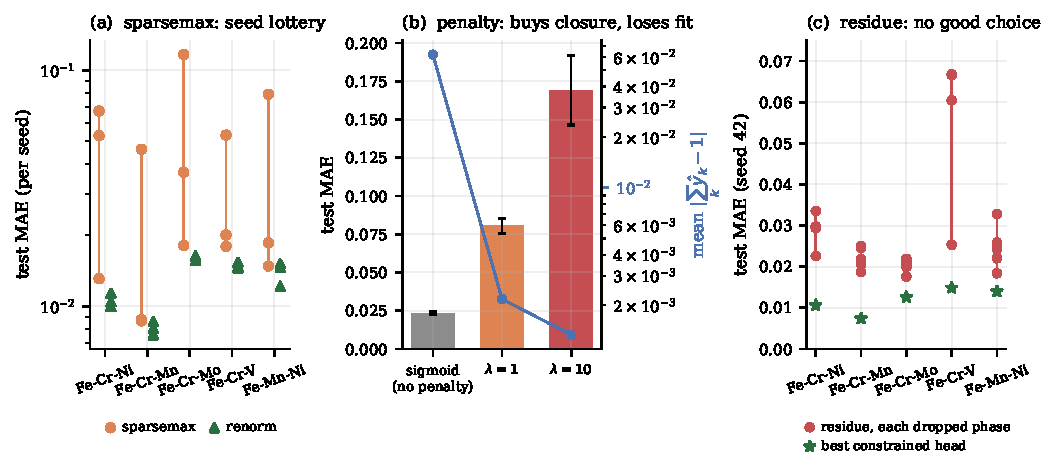
\includegraphics[width=\textwidth]{figures/fig6_failures}
\caption{Three negative results. (a) Sparsemax: per-seed test MAE (orange)
versus the renorm head (green) across all five systems. The seed-to-seed
spread of sparsemax is of the same order as its mean. (b) Sum-to-one penalty
on Fe--Cr--Ni: MAE (bars, left axis) and closure violation (line, right axis)
as $\lambda$ increases. The penalty buys closure at the cost of the fit.
(c) Residue sweep: per-phase MAE for each choice of dropped phase (red)
versus the best constrained head (green star) across all five systems.}
\label{fig:failures}
\end{figure}

% ======================================================================
\section{Predicted phase fields}
\label{sec:fields}

Figure~\ref{fig:fields} shows the predicted phase-fraction fields for
Fe--Cr--Ni under the renorm head, alongside the CALPHAD oracle, for all four
target phases. The surrogate reproduces the phase-boundary structure --- the
BCC, FCC, liquid and sigma fields --- with visible accuracy. The error panel
shows that errors concentrate at phase boundaries, where the fraction changes
rapidly, and are small in the interior of single-phase fields.

We quantified this concentration on the Fe--Cr--Ni test set. For each row
we computed the distance, in scaled $(x_2, x_3, T)$ coordinates, to the
nearest test row with a different active-phase set (a KD-tree boundary
proxy; a differing set was found within 64 neighbours for 92.9\% of rows),
and binned the per-row mean absolute error by that distance. This proxy
measures proximity to regions where the active-phase set changes in the
sampled data; it is not the exact thermodynamic distance to a phase
boundary. Rows in the
nearest third to the boundary proxy carry a mean MAE of 0.022, against 0.008
in the middle third and 0.002 in the farthest third --- a boundary-to-interior
ratio of $\sim$10$\times$. In this system, surrogate error is strongly
concentrated near regions where the active-phase set changes, while the
interior of phase fields is reproduced to high accuracy.

\begin{figure}[htbp]
\centering
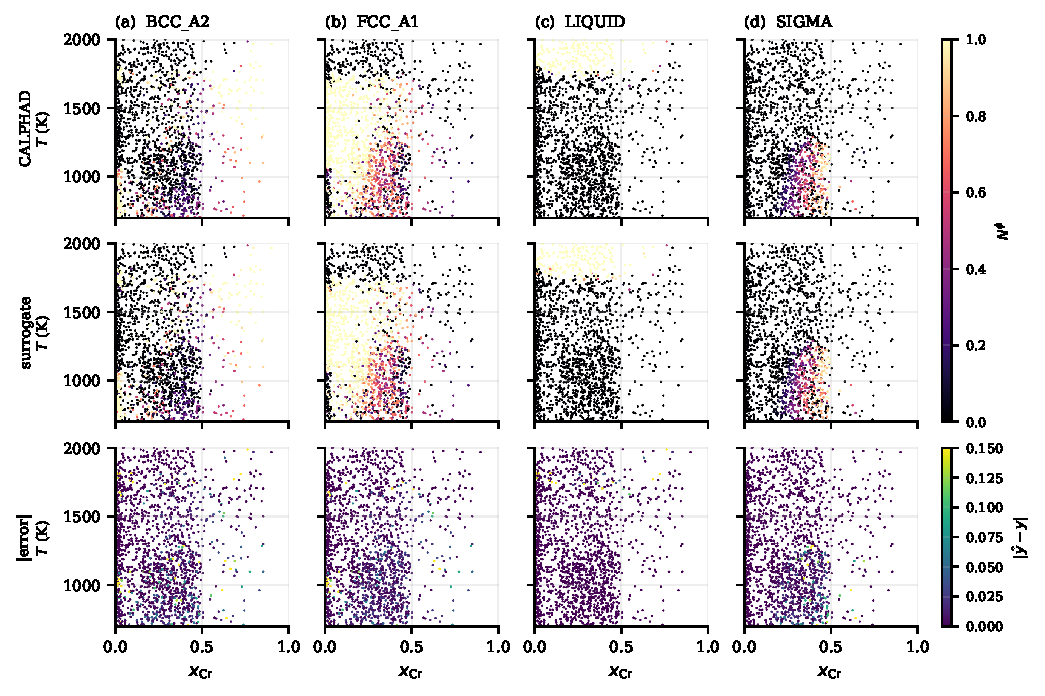
\includegraphics[width=\textwidth]{figures/fig3_fields}
\caption{Predicted phase-fraction fields for Fe--Cr--Ni under the renorm
head (seed 42). Top row: CALPHAD oracle. Middle row: surrogate prediction.
Bottom row: absolute error. Errors concentrate near regions where the
active-phase set changes; the interior of single-phase fields is reproduced
to high accuracy.}
\label{fig:fields}
\end{figure}

% ======================================================================
\section{Discussion}
\label{sec:discussion}

\subsection{When do constrained MLPs beat trees?}

In the five systems studied here, the answer tracked geometry. Systems with
extended smooth coexistence fields --- Fe--Cr--Ni, Fe--Cr--Mn, and to a
lesser extent Fe--Cr--Mo --- favoured the smooth function class of the MLP.
Systems dominated by sharp, essentially binary phase boundaries ---
Fe--Cr--V, Fe--Mn--Ni --- favoured axis-aligned tree splits. We present
this as an empirical observation across the tested systems, not a universal
law: with only five systems, system identity is confounded with phase
topology, rare-phase frequency, sampling density, and boundary geometry.
A surrogate pipeline should evaluate both families and select per system;
no single evaluated architecture consistently dominated across the five
systems.

\subsection{The spatial-generalisation result reframes the interpolation
comparison}

The holdout results of Section~\ref{sec:extrapolation} reframe the main
comparison. On Fe--Cr--Ni the MLP leads the random forest by 41\% on the
interpolation split; on the contiguous composition band the gap widens to
$3.11\times / 1.61\times \approx 1.9\times$ in penalty ratio, and the same
ordering persists under the tested strict one-sided extrapolation
protocols. The MLP's advantage is not merely that it fits the training
distribution better; within the tested protocols it also degrades less
severely in absolute error when the query point leaves it. We do not claim
that the MLP extrapolates reliably: all evaluated model families degrade
sharply in absolute terms, and the MLP's advantage is one of relative
degradation. For alloy-design workflows that query unseen compositions,
this relative comparison is the more relevant one.

\subsection{What the surrogate is and is not}

The surrogate emulates the oracle: for a queried $(\mathbf{x}, T)$ it returns
the phase fractions the database's equilibrium routine would return, fast.
It inherits the oracle's assumptions --- the database's Gibbs energies, the
equilibrium assumption itself, and the solver's convergence behaviour. It is
not an independent thermodynamic statement. ``Validated against the database''
here means ``reproduces the database's answers to solver precision on the
validated points'', not ``thermodynamically true''.

\subsection{Limitations}

Phase-set sufficiency is validated on 1{,}500 re-solved points, not proven
for the whole design space; a phase active only inside an unprobed region
would be missed, and the phase basis itself was fixed with knowledge of the
whole sampled domain, so all results are conditional on this globally
predefined phase basis and do not assess discovery of previously unseen
phases (Section~\ref{sec:data}). The contiguous-band holdout
is a missing-region test inside the sampled domain; the strict
extrapolation protocol is one-sided and covers only one coordinate at a
time, and behaviour beyond the sampled simplex remains unvalidated. The
sparsemax and penalty conclusions are scoped to the tested hyperparameters.
The design distribution is deliberately structured, not uniform, so all
reported average errors are expectations under that sampling distribution;
rankings could shift under a different prior. All MLPs share one fixed
architecture and all baselines use fixed hyperparameters; the comparison is
a fixed-protocol benchmark, not an exhaustive hyperparameter search, and
the reported MLP is not architecture-optimal. The mean $\pm$ standard
deviation over three seeds quantifies seed-to-seed training stochasticity
only, not total predictive uncertainty. The phase-boundary analysis uses an
empirical boundary proxy, not the exact thermodynamic distance to a phase
boundary. Finally, the comparison set is not
exhaustive over function classes: classical low-dimensional interpolants
such as radial-basis-function or spline fits, or Gaussian-process
regression, might approximate these three-dimensional phase-fraction fields
competitively, and we did not evaluate them; the $k$-NN baseline partially
covers the local-smoothness regime. Compositional-data-analysis regressors
such as log-ratio (ALR/CLR/ILR) regression and Dirichlet regression are
likewise not evaluated: the targets contain structural zeros --- only one
to three of the $K$ phases are active on any given row --- and log-ratio
transforms require strictly positive components, so these families would
need ad hoc zero replacement before fitting.

% ======================================================================
\section{Conclusions}
\label{sec:conclusions}

We compared simplex-constraint mechanisms for neural-network phase-fraction
prediction --- six output heads across all five systems plus two mechanism
probes --- against four classical baselines across five Fe-based ternary
systems, totalling 44{,}397 mass-balance-validated equilibria. The
contribution is a systematic empirical benchmark with controls, not a new
architecture.

Structurally constrained heads --- softmax, sigmoid/$\Sigma$, and renorm ---
satisfy the full simplex constraint (closure and non-negativity) to float32
precision at no accuracy cost relative to the unconstrained sigmoid, which
violates closure by 6--8\%. The residue head enforces closure by
construction but not non-negativity, emitting negative fractions on up to
1.2\% of cells. Post-hoc renormalisation repairs all evaluated models to machine
precision and did not hurt accuracy in any of the five systems tested.

No single evaluated architecture consistently dominated across the five
systems. In the systems studied here, constrained MLPs led where dense
smooth coexistence fields dominate; random forests won where sharp
boundaries dominate; paired-bootstrap tests confirmed the two near-ties.

Two spatial protocols with size-matched random controls separated the
spatial penalty from the data-volume penalty. On contiguous interior
holdout bands --- which lie 99.3--99.4\% inside the convex hull of the
remaining training points, and are therefore a distribution-shift test
rather than extrapolation --- the random forest paid $3.11\times$ against
$1.61\times$ for the constrained MLP on the Fe--Cr--Ni composition band,
whereas on the temperature band both paid $1.31\times$: the
temperature-band penalty is largely a data effect. Under strict one-sided
out-of-range extrapolation all evaluated model families degraded sharply,
and the constrained MLP achieved the lowest absolute far-side error in all
five systems, although absolute extrapolation performance remains poor.
Constrained MLPs degrade
more gracefully than trees when queries leave the trained region; graceful
degradation is not reliable extrapolation.

Phase-presence detection degrades faster than regression under distribution
shift: $F_1$ collapses on the held-out temperature band for all evaluated
models even where MAE barely moves. The model with the lowest MAE is not
necessarily the best detector --- regression accuracy and phase-presence
detection are distinct tasks --- and the qualitative gap is stable across
presence thresholds $10^{-4}$--$10^{-2}$, although the detector ranking
flips with the threshold on Fe--Cr--Mo.

Three negative results are informative. Under the evaluated configuration
sparsemax exhibited severe seed sensitivity, consistent with a
zero-gradient sparsity trap. For the tested formulation and $\lambda$
values, a sum-to-one penalty was redundant and strongly detrimental. The
residue head, which closes the sum algebraically, is 1.3--2.5$\times$
worse than the best constrained head in all five systems, consistent with the
residual phase absorbing the accumulated error of the other channels.

% ======================================================================
\section*{Data availability}

The generation pipeline validates mass balance at acceptance time, and all
figures and tables are generated programmatically from stored result
artefacts; no reported value is hand-entered. The recompute audit re-derives
every metric from the stored prediction tensors and confirms agreement to
$<10^{-9}$ on all seven summary fields for all 99 MLP runs.

% ======================================================================
\bibliographystyle{elsarticle-harv}
\begin{thebibliography}{99}

\bibitem[Saunders and Miodownik(1998)]{saunders1998calphad}
Saunders, N., Miodownik, A.P., 1998. CALPHAD: A Comprehensive Guide. Pergamon,
Oxford.

\bibitem[Lukas et al.(2007)]{lukas2007computational}
Lukas, H.L., Fries, S.G., Sundman, B., 2007. Computational Thermodynamics: The
Calphad Method. Cambridge University Press.

\bibitem[Otis and Liu(2017)]{pycalphad}
Otis, R., Liu, Z.-K., 2017. pycalphad: CALPHAD-based computational
thermodynamics in Python. J. Open Res. Softw. 5, 1.

\bibitem[Hart et al.(2021)]{hart2021fast}
Hart, G.L.W., Mueller, T., Toher, C., Curtarolo, S., 2021. Machine learning for
alloys. Nat. Rev. Mater. 6, 730--755.

\bibitem[Nentwich and Engell(2019)]{nentwich2019surrogate}
Nentwich, C., Engell, S., 2019. Surrogate modeling of phase equilibrium
calculations using adaptive sampling. Comput. Chem. Eng. 126, 204--217.

\bibitem[Jiang et al.(2019)]{jiang2019fast}
Jiang, X., Zhang, R., Zhang, C., Yin, H., Qu, X., 2019. Fast prediction of the
quasi phase equilibrium in phase field model for multicomponent alloys based
on machine learning method. Calphad 66, 101644.

\bibitem[Tahkola et al.(2026)]{tahkola2026accelerated}
Tahkola, M., Linnala, L., Blackburn, T., Savukoski, S., Gagneur, V.,
Kaipainen, J., Ma, K., Knowles, A.J., Laukkanen, A., Pinomaa, T., 2026.
Accelerated discovery of Cr-based A2+B2 superalloys across 11 elements with
a deep-learning CALPHAD surrogate. npj Comput. Mater.
\url{https://doi.org/10.1038/s41524-026-02113-x}.

\bibitem[Feng et al.(2021)]{feng2021general}
Feng, S., Fu, H., Zhou, H., Wu, Y., Lu, Z., Dong, H., 2021. A general and
transferable deep learning framework for predicting phase formation in
materials. npj Comput. Mater. 7, 22.

\bibitem[Lu et al.(2024)]{lu2024classified}
Lu, J., Xu, G., Chen, F., Cui, Y., 2024. Classified dataset, regression and
machine learning modeling for prediction of phase transformation
temperatures in steels. Calphad 87, 102748.

\bibitem[Wang and Xiong(2020)]{wang2020uncertainty}
Wang, X., Xiong, W., 2020. Uncertainty quantification and composition
optimization for alloy additive manufacturing through a CALPHAD-based ICME
framework. npj Comput. Mater. 6, 188.

\bibitem[Chen and Guestrin(2016)]{chen2016xgboost}
Chen, T., Guestrin, C., 2016. XGBoost: A scalable tree boosting system. Proc.
KDD, 785--794.

\bibitem[Breiman(2001)]{breiman2001random}
Breiman, L., 2001. Random forests. Mach. Learn. 45, 5--32.

\bibitem[Martins and Astudillo(2016)]{martins2016sparsemax}
Martins, A.F.T., Astudillo, R.F., 2016. From softmax to sparsemax: A sparse
model of attention and multi-label classification. Proc. ICML, 1614--1623.

\bibitem[MatCalc(2023)]{matcalc}
MatCalc, 2023. Open thermodynamic databases.
\url{https://www.matcalc.at/}. Accessed 2024.

\end{thebibliography}

\end{document}
